\chapter{Keynote speakers}
\section{About the Why? and the How? of psychologically plausible agents}

\noindent \textit{Prof. Dr. Andreas Ernst}

\noindent December 5, 09:00-10:00
\\

\noindent To deepen the analysis and understanding of human behaviour by
using artificial societies, a credible modelling of agents and their decision
processes is needed. Such a deep analysis can be informed by the psychological
knowledge about processes and triggers of specific behaviours, given the
interaction between an agent’s environment and some individual preference set.
This requires a framework capable of handling a high number of deep,
heterogeneous agents, together with their individual networks.

In this presentation, a software framework is presented that aims at providing
psychological plausibility to the modelling of so-called citizen agents. It
fills the gap between (flat) agent frameworks without any built-in psychological
foundations on the one hand and full-fledged (deep) cognitive architectures on
the other hand, the latter being computationally too intensive to be of any use
in larger scale problems. The framework provides prefabricated components of an
agent’s decision process like perception, memory, different modes of decision
making, basic learning algorithms, or social influence. Each of these components
is based on appropriate psychological empirical results or theories.

Using this framework, together with specifically gathered data, an agent’s
interaction with other agents, technology, or the natural environment can be
investigated. Examples include energy use, innovation adoption, or helper
networks. Besides the emerging macro phenomena, their micro foundation lying in
the individual preferences and processes are important data produced by the
framework. Individual, local perception of the technical or physical environment
and the information of the individual social network are crucial in determining
an agent’s behaviour.

To model larger amounts of social data, with a higher number of agents together
with their networks, the sociological concept of lifestyles can be used as a
classifying element, and as a bridge to upscale the individual data to the agent
set.\\

\begin{wrapfigure}[13]{l}{11em}
  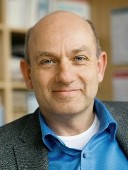
\includegraphics{andreas_ernst}
\end{wrapfigure}
\noindent\textbf{Andreas Ernst} achieved his psychology Diplom
degree with a focus on psychology of knowledge/cognitive science in 1988. He
finished his PhD—entitled "Social knowledge as basis of decisions in conflict
situations"—in 1993. Until 1999 he was assistant professor at the Institute of
Psychology, University of Freiburg i. Br. and in the same year he finished his
postdoctoral lecture qualification under the title: "Information dilemmas and
the use of natural resources". After another three years at the Institute of
Psychology, University of Freiburg i.Br. he became full professor for
Environmental Systems Analysis at the Center for Environmental Systems Research
of the University of Kassel. He also heads the Graduate Program
"Man-Environment-Systems" (ProMUS) and is the current president of the European
Social Simulation Association (ESSA). Prof. Dr. Andreas Ernst is co-editor of
the book series "Social Science Simulations" of the Metropolis-Verlag.


\section{Big Data and the Attention Economy}

\noindent \textit{Bernardo A. Huberman}

\noindent December 6, 09:00-10:00
\\

\noindent The advent of the web has led to an ever expanding ocean of data whose
outlines are hard to discern but its effects are easy to feel. It reflects a
societal change that is both global and daunting at the same time. Global
because it encompasses content created by people seeking attention and
information from all over the world without much awareness of privacy issues.
And daunting since it is hard to discern what to pay attention to when
confronted with such flood of content.

This talk will describe the effects that the attention economy has on the
production and consumption of big data and the opportunities that big data
offers about learning the behavior of large groups of people and the design of
novel socially attentive systems. It will also address the questions that big
data poses about privacy and how markets for private data can restore a sense of
control to most users of the web.\\

\begin{wrapfigure}[13]{l}{11em}
  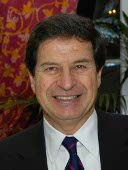
\includegraphics{bernardo_huberman}
\end{wrapfigure}

\noindent\textbf{Bernardo A. Huberman} is a Senior HP Fellow and director of
the Social Computing Research Group at HP Labs, which focuses on methods for
harvesting the collective intelligence of groups of people in order to realize
greater value from the interaction between users and information. Huberman’s
main research focus is on the relationship between local actions and the global
behavior of large, distributed systems. Areas of exploration include distributed
knowledge, social organizations and the economics of attention. Much of
Huberman's research has concentrated on the World Wide Web, with an emphasis on
the dynamics of its growth and use. This work helped uncover the nature of
electronic markets, the detailed structure of the web and the laws governing the
way people surf for information. One of the originators of the field of ecology
of computation, Huberman recently published the book, "The Laws of the Web:
Patterns in the Ecology of Information," with MIT Press.

\section{From Computational Social Science to Socio-Inspired Technology to
Artificial Societies}

\noindent \textit{Dirk Helbing}

\noindent December 7, 09:00-10:00
\\

\noindent  What can we learn from the way society is organized? What are the
underlying principles? How can we use them to design new technological systems?

Along the lines of these guiding questions, I will start with models of
pedestrians and crowds, and the applications in logistics and traffic light
control they have inspired.

It will be shown that self-organization is a wide-spread principle underlying
the emergence of social coordination, cooperation, and social norms. These
phenomena can now be dynamically modeled based on evolutionary principles, which
are transferable to ICT systems as well. I will also discuss, how and why the
wrong kinds of system designs can lead to breakdowns of traffic flows,
cooperation, or financial markets. It will be argued that the theory of complex
systems can help to provide an explanatory understanding of desirable and
undesirable cascading effects and guidelines for the design of socially
interactive systems (such as the 'ecosystem' of financial trading algorithms).
\\

\begin{wrapfigure}[13]{l}{11em}
  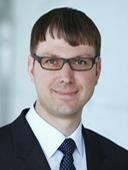
\includegraphics{dirk_helbing}
\end{wrapfigure}

\noindent\textbf{Dirk Helbing} has worked as Managing Director of the Institute
for Transport \& Economics at TU Dresden and is now Professor of Sociology, in
particular of Modeling and Simulation at ETH Zurich. Having studied physics and
mathematics, he investigates complex social, economic, and transport systems
with methods from statistical physics, individual-based models, and behavioral
experiments. Helbing is well-known for the social force model, in particular its
application to self-organization phenomena in pedestrian crowds. Besides the
slower-is-faster effect, he introduced the freezing-by-heating effect and the
phase diagram of congested traffic states. Recent work applies principles of
collective intelligence and dynamics to the optimization of freeway and urban
traffic flows. In game theory, Helbing proposed a microscopic foundation of
evolutionary game theory and studied self-organized behavioral conventions early
on. His current work develops socio-inspired technologies and investigates the
role of success-driven motion for the establishment of cooperation among selfish
individuals.
